\clearpage

\chapter{Sequenzdiagramme}

\section{Sequenzdiagramm  zu T20}

Im folgenden Diagramm wird der Ablauf zu unserem Testfall T20, dem allgemeinen Start der App, dargestellt. Der User klickt hierzu auf das App-Symbol und ruft dadurch den Android-Launcher auf, welcher eine neue Instanz von RetroMachines erstellt und deren Attribute initialisiert bzw. das schon gespeicherte Spiel lädt. Der Ladebildschirm erscheint als erster Screen, sobald der Ladevorgang abgeschlossen ist, wird der Anwender zur Benutzerverwaltung weitergeleitet, um eines der Spielerprofile als aktiv auszuwählen. Danach wird er ins Hauptmenü weitergeleitet.

\begin{figure}[!htb]
	\centering
	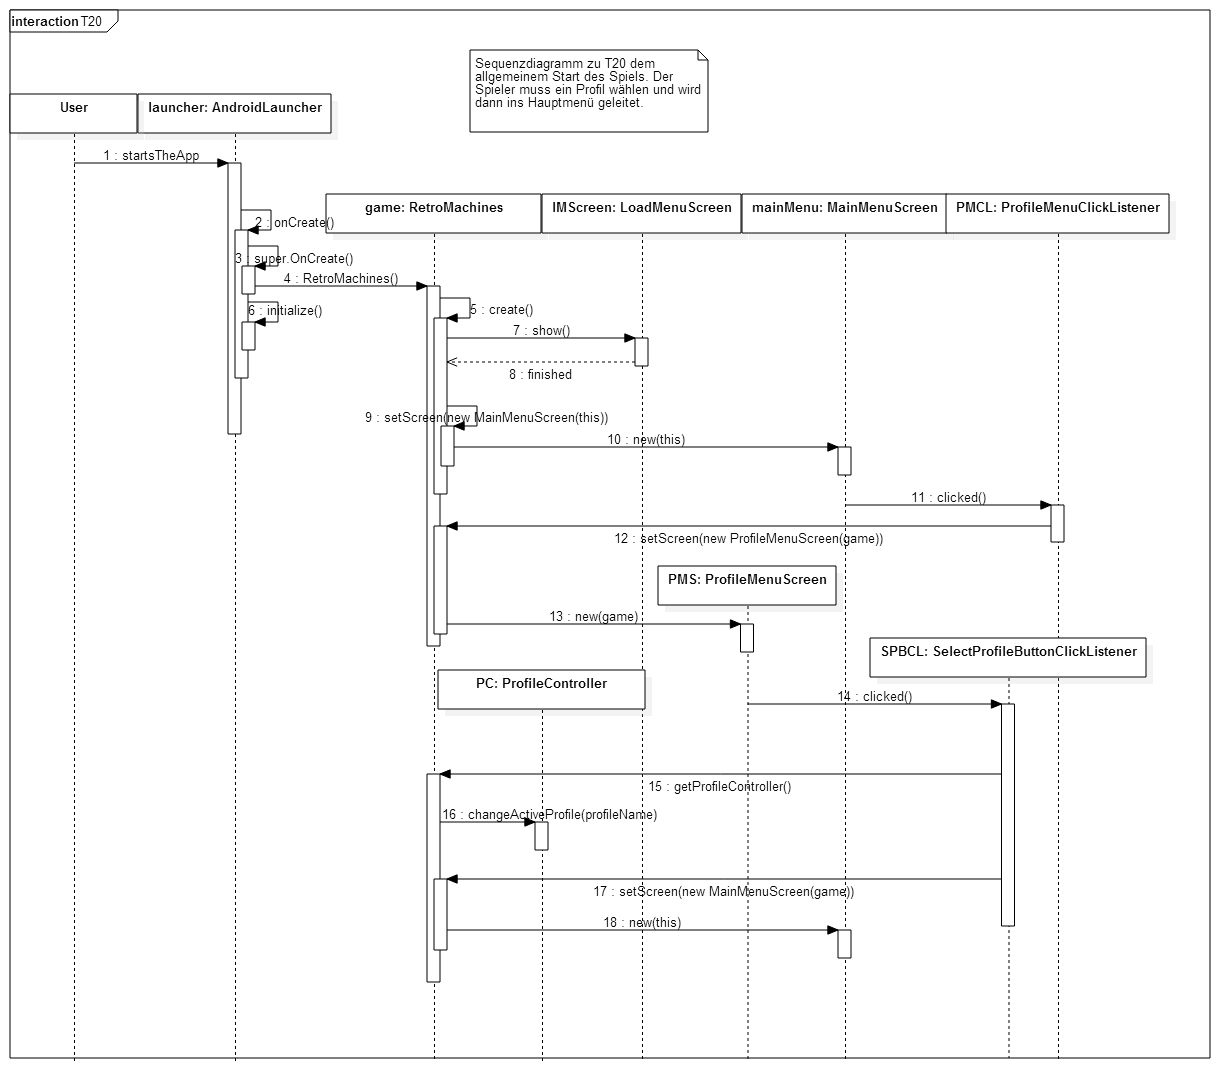
\includegraphics[width=1\textwidth]{../../images/T20.png}
	\caption{T20}
	\label{fig:t100evluation}
\end{figure}

\section{Sequenzdiagramm zu T100 (Level spielen)}

Der Anwender befindet sich beim Start dieses Diagrammes im Levelmenü. Durch Drücken auf ein Levelsymbol wählt er das entsprechende Level zum Spielen aus und der GameScreen wird angezeigt. Im Folgenden reagiert die Spielfigur auf das Drücken der Buttons \enquote{nach rechts}, \enquote{nach links}, \enquote{springen} und kann - sofern sie sich neben einem Objekt befindet - dieses aufnehmen und danach wieder ablegen, solange sie noch nichts trägt.

\begin{figure}[!htb]
    \centering
    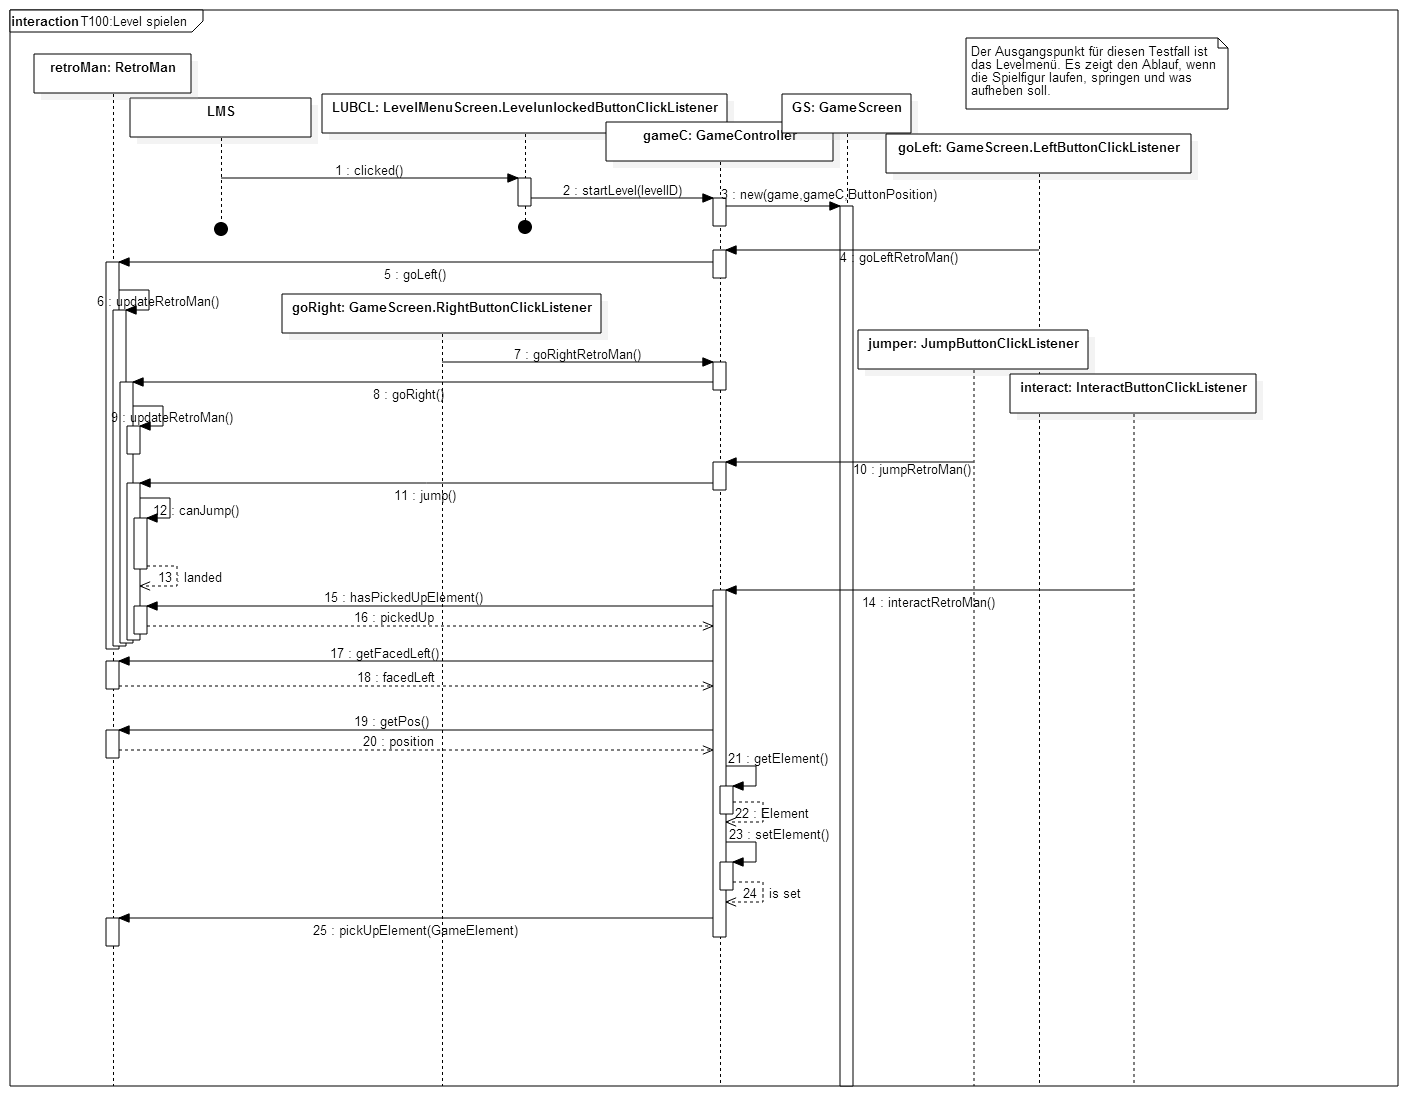
\includegraphics[width=1\textwidth]{../../images/T100_Level_spielen.png}
    \caption{T100 Level spielen}
    \label{fig:t100evluation}
\end{figure}


\section{Sequenzdiagramm zu T100 (Evaluation)}


Nachdem alle Spielelemente in den Ablagen platziert sind, kann der Anwender den Button \enquote{Evaluation starten} betätigen. Falls die Elemente richtig platziert sind, startet die Animation der Auswertung, während der keine Benutzereingaben möglich sind; falsche Lambda-Konstrukte werden nicht ausgewertet. Hierzu wird die zugehörige  Baumstruktur zum Lambda-Term aufgebaut und anschließend die Beta-Reduktion und Alpha-Konversion schrittweise angewandt.

\begin{figure}[!htb]
	\centering
	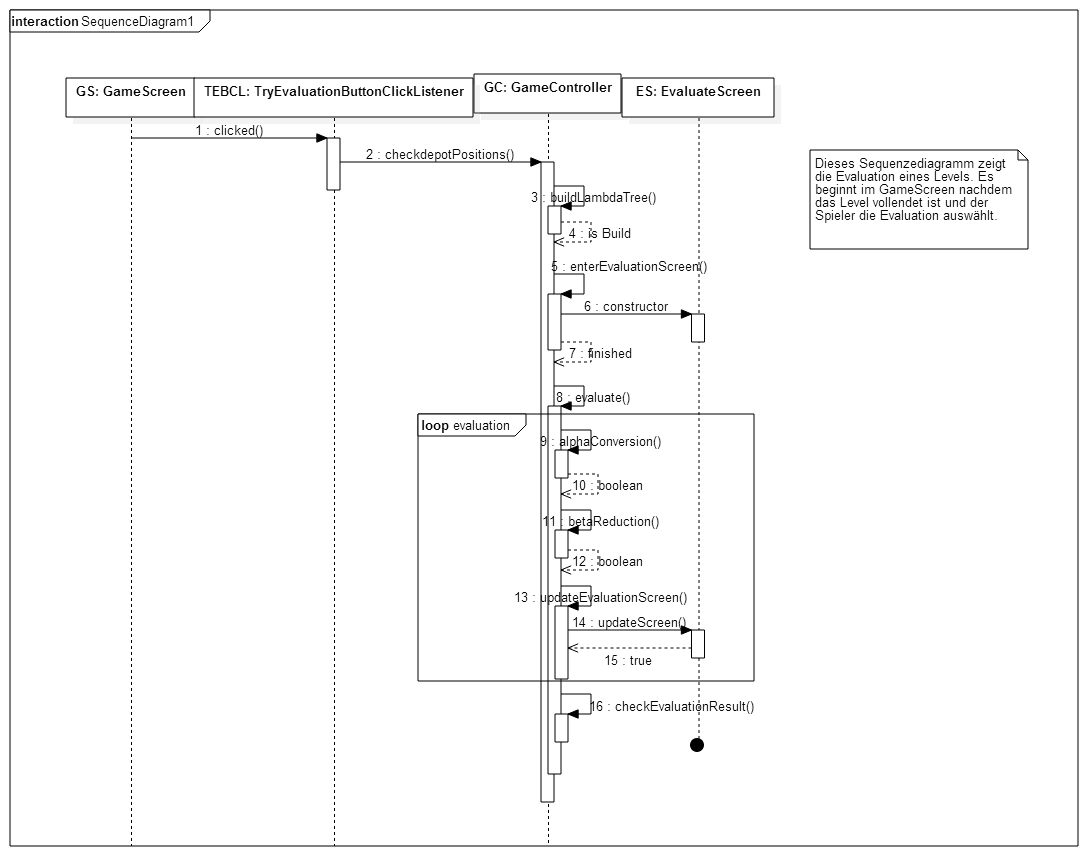
\includegraphics[width=1\textwidth]{../../images/T100Evaluation.png}
	\caption{T100 Evaluation}
	\label{fig:t100evluation}
\end{figure}


\section{Sequenzdiagramm zu T40}

Um ein neues Profil zu erstellen, muss im Profilmenü auf den \enquote{+}-Button geklickt werden; um durch die bestehenden Profile zu scrollen, können \enquote{Hoch}- und \enquote{Runter}-Buttons betätigt werden. Infolgedessen öffnet sich eine neue Anzeige, in welcher der User seinen Namen eingibt und Avatar sowie Links- oder Rechtshändersteuerung auswählt. Durch den \enquote{Ok}-Button bestätigt er das Profil und es wird zur bestehenden Datenstruktur hinzugefügt, der Anwender wird zurück ins Profilmenü geleitet.

\begin{figure}[!htb]
    \centering
    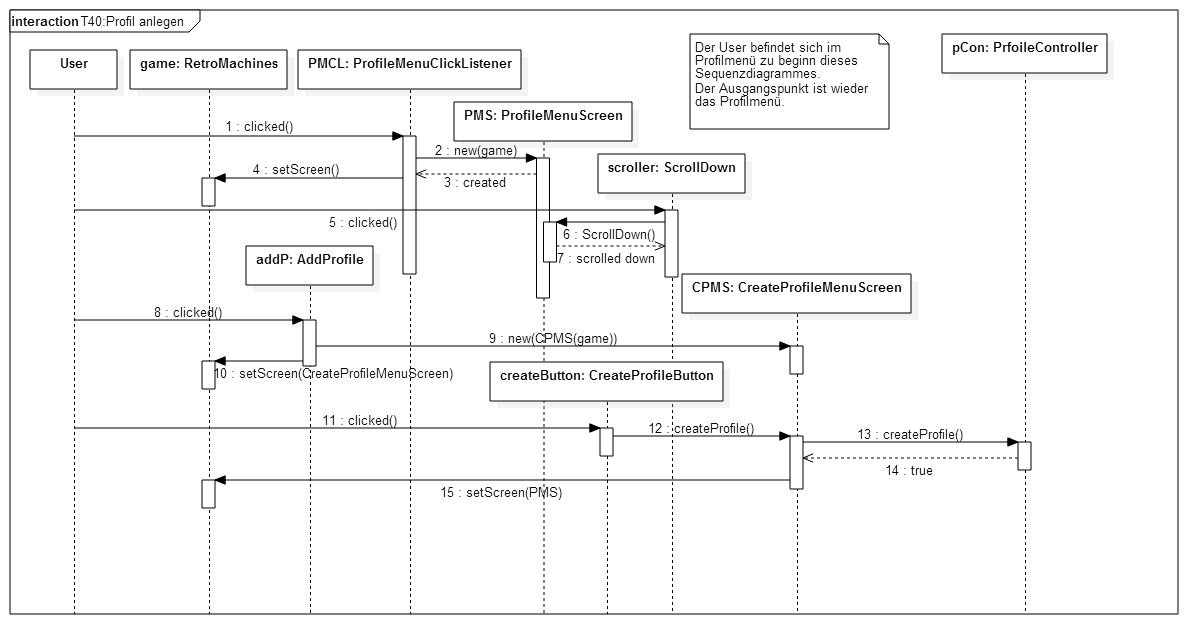
\includegraphics[width=1\textwidth]{../../images/T40_Profil_anlegen.png}
    \caption{T40}
    \label{fig:t100evluation}
\end{figure}